\iffalse
\documentclass[journal,12pt,twocolumn]{IEEEtran}
\usepackage{setspace}
\usepackage{gensymb}
\singlespacing
\usepackage[cmex10]{amsmath}
\usepackage{amsthm}
\usepackage{mathrsfs}
\usepackage{txfonts}
\usepackage{stfloats}
\usepackage{bm}
\usepackage{cite}
\usepackage{cases}
\usepackage{subfig}
\usepackage{longtable}
\usepackage{multirow}
\usepackage{enumitem}
\usepackage{mathtools}
\usepackage{steinmetz}
\usepackage{tikz}
\usepackage{circuitikz}
\usepackage{verbatim}
\usepackage{tfrupee}
\usepackage[breaklinks=true]{hyperref}
\usepackage{tkz-euclide}
\usetikzlibrary{calc,math}
\usepackage{listings}
    \usepackage{color}                                            %%
    \usepackage{array}                                            %%
    \usepackage{longtable}                                        %%
    \usepackage{calc}                                             %%
    \usepackage{multirow}                                         %%
    \usepackage{hhline}                                           %%
    \usepackage{ifthen}                                           %%
  %optionally (for landscape tables embedded in another document): %%
    \usepackage{lscape}     
\usepackage{multicol}
\usepackage{chngcntr}
\DeclareMathOperator*{\Res}{Res}
\renewcommand\thesection{\arabic{section}}
\renewcommand\thesubsection{\thesection.\arabic{subsection}}
\renewcommand\thesubsubsection{\thesubsection.\arabic{subsubsection}}

\renewcommand\thesectiondis{\arabic{section}}
\renewcommand\thesubsectiondis{\thesectiondis.\arabic{subsection}}
\renewcommand\thesubsubsectiondis{\thesubsectiondis.\arabic{subsubsection}}

% correct bad hyphenation here
\hyphenation{op-tical net-works semi-conduc-tor}
\def\inputGnumericTable{}                                 %%

\lstset{
frame=single, 
breaklines=true,
columns=fullflexible
}

\begin{document}


\newtheorem{theorem}{Theorem}[section]
\newtheorem{problem}{Problem}
\newtheorem{proposition}{Proposition}[section]
\newtheorem{lemma}{Lemma}[section]
\newtheorem{corollary}[theorem]{Corollary}
\newtheorem{example}{Example}[section]
\newtheorem{definition}[problem]{Definition}
\newcommand{\BEQA}{\begin{eqnarray}}
\newcommand{\EEQA}{\end{eqnarray}}
\newcommand{\define}{\stackrel{\triangle}{=}}

\bibliographystyle{IEEEtran}
\providecommand{\mbf}{\mathbf}
\providecommand{\pr}[1]{\ensuremath{\Pr\left(#1\right)}}
\providecommand{\qfunc}[1]{\ensuremath{Q\left(#1\right)}}
\providecommand{\sbrak}[1]{\ensuremath{{}\left[#1\right]}}
\providecommand{\lsbrak}[1]{\ensuremath{{}\left[#1\right.}}
\providecommand{\rsbrak}[1]{\ensuremath{{}\left.#1\right]}}
\providecommand{\brak}[1]{\ensuremath{\left(#1\right)}}
\providecommand{\lbrak}[1]{\ensuremath{\left(#1\right.}}
\providecommand{\rbrak}[1]{\ensuremath{\left.#1\right)}}
\providecommand{\cbrak}[1]{\ensuremath{\left\{#1\right\}}}
\providecommand{\lcbrak}[1]{\ensuremath{\left\{#1\right.}}
\providecommand{\rcbrak}[1]{\ensuremath{\left.#1\right\}}}
\theoremstyle{remark}
\newtheorem{rem}{Remark}
\newcommand{\sgn}{\mathop{\mathrm{sgn}}}
\providecommand{\abs}[1]{\left\vert#1\right\vert}
\providecommand{\res}[1]{\Res\displaylimits_{#1}} 
\providecommand{\norm}[1]{\left\lVert#1\right\rVert}
\providecommand{\mtx}[1]{\mathbf{#1}}
\providecommand{\mean}[1]{E\left[ #1 \right]}
\providecommand{\fourier}{\overset{\mathcal{F}}{ \rightleftharpoons}}
\providecommand{\system}{\overset{\mathcal{H}}{ \longleftrightarrow}}
\newcommand{\solution}{\noindent \textbf{Solution: }}
\newcommand{\cosec}{\,\text{cosec}\,}
\providecommand{\dec}[2]{\ensuremath{\overset{#1}{\underset{#2}{\gtrless}}}}
\newcommand{\myvec}[1]{\ensuremath{\begin{pmatrix}#1\end{pmatrix}}}
\newcommand{\mydet}[1]{\ensuremath{\begin{vmatrix}#1\end{vmatrix}}}
\numberwithin{equation}{subsection}
\makeatletter
\@addtoreset{figure}{problem}
\makeatother

\let\StandardTheFigure\thefigure
\let\vec\mathbf
\renewcommand{\thefigure}{\theproblem}



\def\putbox#1#2#3{\makebox[0in][l]{\makebox[#1][l]{}\raisebox{\baselineskip}[0in][0in]{\raisebox{#2}[0in][0in]{#3}}}}
     \def\rightbox#1{\makebox[0in][r]{#1}}
     \def\centbox#1{\makebox[0in]{#1}}
     \def\topbox#1{\raisebox{-\baselineskip}[0in][0in]{#1}}
     \def\midbox#1{\raisebox{-0.5\baselineskip}[0in][0in]{#1}}

\vspace{3cm}


\title{Assignment 1}
\author{Jaswanth Chowdary Madala}





% make the title area
\maketitle

\newpage

%\tableofcontents

\bigskip

\renewcommand{\thefigure}{\theenumi}
\renewcommand{\thetable}{\theenumi}


\begin{enumerate}

\textbf{Solution:}
\fi
See Table \ref{tab:chapters/9/10/4/4/1}.
Let the equations of two concentric circles be,
\begin{align}
\norm{\vec{x}}^2 &= 4
\label{eq:chapters/9/10/4/4/1}\\
\norm{\vec{x}}^2 &= 9
\label{eq:chapters/9/10/4/4/2}
\end{align}
Consider the line
		\begin{align}
\vec{x} &= \vec{h} + \mu \vec{m}
\label{eq:chapters/9/10/4/4/3}\\
\end{align}
 with parameters
\begin{align}
\vec{h} = \myvec{1\\0}, \, \vec{m} &= \myvec{0\\1}
\label{eq:chapters/9/10/4/4/6}
\end{align} 
Then,
\begin{align}
\mu^2\vec{m}^{\top}\vec{V}\vec{m} + 2 \mu\vec{m}^{\top}\brak{\vec{V}\vec{h}+\vec{u}} 
	+ \text{g}\brak{\vec{h}} &=0
\label{eq:chapters/9/10/4/4/5}
\end{align}
with
\begin{align}
\text{g}\brak{\vec{x}} &= \vec{x}^{\top}\vec{V}\vec{x}+2\vec{u}^{\top}\vec{x}+f=0
\label{eq:chapters/9/10/4/4/4}
\end{align}
Substituting
\begin{align}
\vec{V} = \vec{I}, \, \vec{u} = \vec{O}, \, f &= -4
\end{align}
the points of intersection of circle \eqref{eq:chapters/9/10/4/4/1} and the line \eqref{eq:chapters/9/10/4/4/3} with parameters given by \eqref{eq:chapters/9/10/4/4/6} $\vec{B},\vec{C}$ are given by,
\begin{align}
\mu ^2 - 3 &= 0
\implies \mu = \pm \sqrt{3}
\end{align}
yielding
\begin{align}
\vec{B} = \myvec{1\\\sqrt{3}}, \, \vec{C} &= \myvec{1\\-\sqrt{3}}
\end{align}
Substituting
\begin{align}
\vec{V} = \vec{I}, \, \vec{u} = \vec{O}, \, f &= -9\\
\end{align}
The points of intersection of circle \eqref{eq:chapters/9/10/4/4/2} and the line \eqref{eq:chapters/9/10/4/4/3} with parameters given by \eqref{eq:chapters/9/10/4/4/6} $\vec{A},\vec{D}$ are given by,
\begin{align}
\mu ^2 - 8 &= 0
\implies \mu = \pm 2\sqrt{2}
\end{align}
yielding
\begin{align}
\vec{A} = \myvec{1\\2\sqrt{2}}, \, \vec{D} &= \myvec{1\\-2\sqrt{2}}
\end{align}
Thus,
\begin{align}
\norm{\vec{A}-\vec{B}} 
	&=\norm{\vec{C}-\vec{D}} 
=  2\sqrt{2}-\sqrt{3}
\\
	\implies AB &= CD.
\end{align}
\begin{table}[h]
\centering
%%%%%%%%%%%%%%%%%%%%%%%%%%%%%%%%%%%%%%%%%%%%%%%%%%%%%%%%%%%%%%%%%%%%%%
%%                                                                  %%
%%  This is a LaTeX2e table fragment exported from Gnumeric.        %%
%%                                                                  %%
%%%%%%%%%%%%%%%%%%%%%%%%%%%%%%%%%%%%%%%%%%%%%%%%%%%%%%%%%%%%%%%%%%%%%%

\begin{center}
\begin{tabular}{|c|c|c|}
\hline
\textbf{Parameter}	&\textbf{Description}& \textbf{Value}\\ \hline
$\vec{O}$	&center of both circles&	$\myvec{0\\0}$\\ \hline
$r_1$		&radius of smaller circle&	2\\ \hline
$r_2$		&radius of larger circle&	3\\ \hline
$\vec{h}$	&point on the line&	$\myvec{1\\0}$\\ \hline
$\vec{m}$	&direction vector of the line&	$\myvec{0\\1}$\\ \hline
\end{tabular}
\end{center}

\caption{}
\label{tab:chapters/9/10/4/4/1}
\end{table}
See Fig. 
\ref{fig:chapters/9/10/4/4/1}
\begin{figure}[ht]
\centering
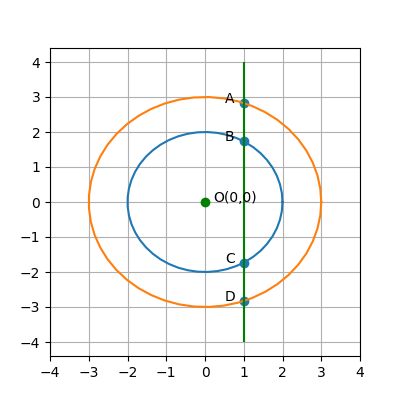
\includegraphics[width = \columnwidth]{chapters/9/10/4/4/figs/fig.png}
\caption{}
\label{fig:chapters/9/10/4/4/1}
\end{figure}
